\part{Use Cases}

%image path:
% ../DesignDocumentation/04_UseCases/


\paragraph{}
%
\includegraphics[height=1in]{useCase_start.jpg} \\

\includegraphics[height=1in]{../DesignDocumentation/04_UseCases/useCase_start.jpg} \\
~\\
\textbf{Name:}  Start
\\ \textbf{Actors:} Client, Server
\\ \textbf{Precondition:} None
\\ \textbf{Trigger:} Some one desires to start the game
\\ \textbf{Main Flow:} 
\begin{enumerate}
	\item The server is started and program launched
	\item The clients are started and programs launched
	\item Clients attempt to connect to server
	\item Server makes connections, remembering order that they were made
	\item Server assigns pieces based on connection order
	\item Server creates a board
	\item Server randomizes cards, keeps a room, weapon, and person card
	\item Server distributes other cards
	\item Server sends board to clients
	\item Server sends message to first connection beginning game play
\end{enumerate}
\textbf{Exceptional Flow:}  Network error or server error
\\ \textbf{Alternate Flow:}  Error, not enough players joined
\\ \textbf{Post-condition:}  Game play in progress
\\ \textbf{Author/Date:}  Green Team, September 29, 2008; revised October 6, 2008
%\\* \\ 
\newpage

%
\includegraphics[height=1in]{useCase_move.jpg} \\

\includegraphics[height=1in]{../DesignDocumentation/04_UseCases/useCase_move.jpg} \\
~\\
\textbf{Name:}  Move
\\ \textbf{Actors:} Server and Client
\\ \textbf{Precondition:} Game play in progress, player�s turn
\\ \textbf{Trigger:} Previous move over message received by server
\\ \textbf{Main Flow:} 
\begin{enumerate}
	\item Sever generates a random integer between 1 and 6
	\item Server computes all (out of a room, into a room, through passage, or along corridor) possible ending spaces from player�s current position
	\item Server sends client updated board
	\item Client chooses end position
	\item Client sends position to server
	\item Server updates game board
	\item Server updates board for all players
\end{enumerate}
\textbf{Exceptional Flow:}  Network error
\\ \textbf{Alternate Flow:}  None
\\ \textbf{Post-condition:}  Turn continues (guess may be possible) (accuse may be possible)
\\ \textbf{Author/Date:}  Green Team, September 29, 2008; revised October 6, 2008
\newpage

%\includegraphics[height=1in]{useCase_guess.jpg} \\
\includegraphics[height=1in]{../DesignDocumentation/04_UseCases/useCase_guess.jpg} \\
~\\
\textbf{Name:}  Guess
\\ \textbf{Actors:} Server and Client
\\ \textbf{Precondition:} Player�s turn and located in a room that they haven�t guessed while being in on this turn
\\ \textbf{Trigger:} Player selects guess button
\\ \textbf{Main Flow:} 
\begin{enumerate}
	\item A form appears over the client GUI containing radio buttons for each player, room, and weapon
	\item Player selects a combination of one weapon, one player, and the current room is pre-selected and unchangeable
	\item Combination is sent to server
	\item Server moves guessed player�s piece to guessed room
	\item Server looks up player cards for first match in order of joining
	\item A player that has a match is queried to show the match or one if they have multiple
	\item That card is shown to guessing player along with which player had it
	\item All players notified of guess made, what the guess was and that it was disproved
	\item Updated board is sent to all players
\end{enumerate}
\textbf{Exceptional Flow:}  Network error
\\ \textbf{Alternate Flow:}  Server is unable to find a match among other players
\begin{itemize}
	\item Message returned to guessing player that no match was found
	\item All players notified that a guess was made, what the guess was, and that it couldn�t be disproved
\end{itemize}
\textbf{Post-condition:}  Game state is updated to reflect changes 
\\ \textbf{Author/Date:}  Green Team September 29, 2008; revised October 6, 2008
\newpage

%\includegraphics[height=1in]{useCase_accusation.jpg} \\
\includegraphics[height=1in]{../DesignDocumentation/04_UseCases/useCase_accusation.jpg} \\
~\\
\textbf{Name:}  Accusation
\\ \textbf{Actors:} Server and Client
\\ \textbf{Precondition:} Player�s turn
\\ \textbf{Trigger:} Player selects accuse button
\\ \textbf{Main Flow:} 
\begin{enumerate}
	\item A form appears over the client GUI containing a radio buttons for each player, room, and weapon
	\item Player selects a combination of one weapon, one player, and one room
	\item Combination is sent to server
	\item Server verifies against saved cards
	\item Server updates game board for all player with game over message, player name has won
	\item Server closes connections to players
	\item Server resets itself, waits for connections
\end{enumerate}
\textbf{Exceptional Flow:}  Network error
\\ \textbf{Alternate Flow:}

	\begin{description}
		\item[Server] finds the combo to not match.
		\begin{itemize}
			\item Player�s status is changed to show cards only status.
			\item Server sends message to players that this player made a wrong accusation, what it was, and that the player is out 
		\end{itemize}
	\end{description}
	
	\begin{description}		
		\item[Server] finds the combo to not match and this is the last active player
		\begin{itemize}
			\item Server sends a message to all players telling them off
			\item Server closes connections to players
			\item Server resets itself
		\end{itemize}
	\end{description}

\textbf{Post-condition:}  Game ends or next player�s turn, server get mad and game ends
\\ \textbf{Author/Date:}  Green Team, September 29, 2008; revised October 6, 2008
